\documentclass{article}
\usepackage[utf8]{inputenc}
\usepackage[T1]{fontenc}

\usepackage{graphicx}
\usepackage{subcaption}

\usepackage{ifxetex}
\ifxetex
  \usepackage{fontspec}
\else
  \usepackage[T1]{fontenc}
  \usepackage[utf8]{inputenc}
  \usepackage{lmodern}
\fi

\title{Reporte de Actividad 9}
\author{Roberto Benard Orci}
\date{28/04/2018}

\begin{document}
\maketitle

\section*{wxMaxima}

wxMaxima es un sistema de álgebra computacional que permite a un usuario escribir
álgebra, cálculo y preguntas estadísticas.

\section{Introducción}

\subsection{Texto}

Para escribir texto uno puede simplemente empezar a escribir o hacer clic en el menú superior, en celda, y seleccionar el tipo de texto que desea escribir. También, uno puede usar atajos, por ejemplo la tecla \textit{Ctrl}.

Aquí hay unos cuantos atajos: \textit{Ctrl} + \textit{1}, \textit{Ctrl} + \textit{2}, \textit{Ctrl} + \textit{3}, \textit{Ctrl} + \textit{4}, y \textit{Ctrl} + \textit{5}, los cuales sirven para ingresar texto, titulo, subtitulo, y subsubtitulo respectivamente.

\begin{center}
	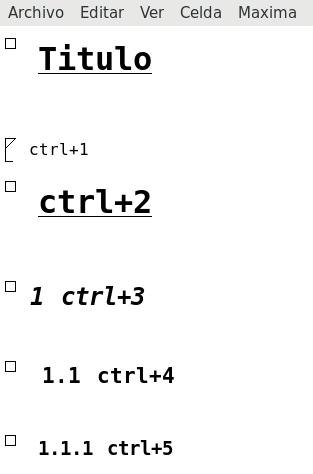
\includegraphics[width=5cm]{texto.png}
    
\end{center}
\vspace{0.3cm}



\subsection{Matemática}

Si escribes cualquier cosa fuera de una celda de texto wxMaxima interpretara esto como una entrada en la que se necesita hacer algo.



\section{Aritmética}

Para hacer cálculos simples unjo simplemente escribe lo que se quiere calcular. Para realizar el calculo uno simplemente presiona \textit{shift} + \textit{Enter}, si uno quiere realizar diferentes cálculos al mismo tiempo uno tiene que separarlos con \textit{;} para poder realizar los cálculos.

\vspace{0.3cm}

Si uno desea utilizar el resultado obtenido en un calculo anterior, puede utilizarlos usando la variable con la que se nombro al resultado, esta aparece a su izquierda  y siempre aparecen con \% seguido de un número. 

\vspace{0.3cm}

Digamos que harás una operación muy grande, o obtendrás muchos valores los cuales no te interesan conocer ya que solo los usaras para obtener otros, para no ver los resultados de esos cálculos simplemente escribe \$ al final de la operación.

\vspace{0.3cm}

wxMaxima te regresara una fracción siempre que sea posible, si quieres los decimales asegúrate de escribir \textit{float(}operación\textit{)}.

\begin{center}
	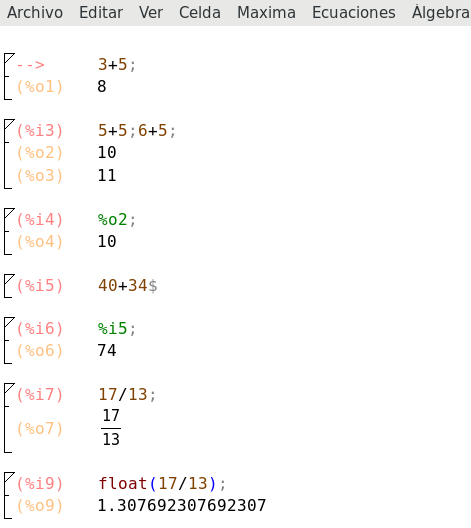
\includegraphics[width=8cm]{Aritmetica.png}
    
\end{center}
\vspace{0.3cm}



\section{Variables, funciones, y ecuaciones}

Si uno desea guardar un número en una variable para operar con ella, escribirá la variable seguido del signo \textit{:}, y después el número que deseas guardar.

Para nombrar una variable con el propósito de verla en diferentes operaciones usa \textit{=} en lugar de \textit{:}.

\vspace{0.3cm}

Si deseas borrar el valor de la variable que guardaste, simplemente escribe \textit{kill(}variable\textit{)}

\vspace{0.3cm}

Al expresar una función de la forma \textit{f(x)=Función} uno no puede igualarla con \textit{:} ni con \textit{=}, si no con \textit{:=}. Una vez guardada, podrás evaluar esta función y hacer operaciones con ella. ¡También puedes hacer composiciones de funciones! no necesariamente tiene que ser \textit{f(x)}.

De la misma manera que puedes nombrar variables y funciones tambien puedes hacer lo mismo con ecuaciones utilizando \textit{:}.

\vspace{0.3cm}

Un comando muy útil es el comando \textit{subst(x=y,g(x))}, en el cual puedes sustituir un número, una variable o una ecuación en otra, primero igualas la variable de la ecuación a la que le quieres sustituir un valor el número/variable/ecuación que quieres sustituir, después una coma, seguido de la ecuación a la que se lo quieres sustituir.




\section{Gráficas}

Graficar es tan sencillo como poner \textit{wxplot2d(f(x),[x,xmin,xmax])}, donde \textit{f(x)} es la función que quieres graficar, \textit{x} es la variables, y \textit{xmin} y \textit{xmax} representan el rango de la variable.

\vspace{0.4cm}
\begin{center}
	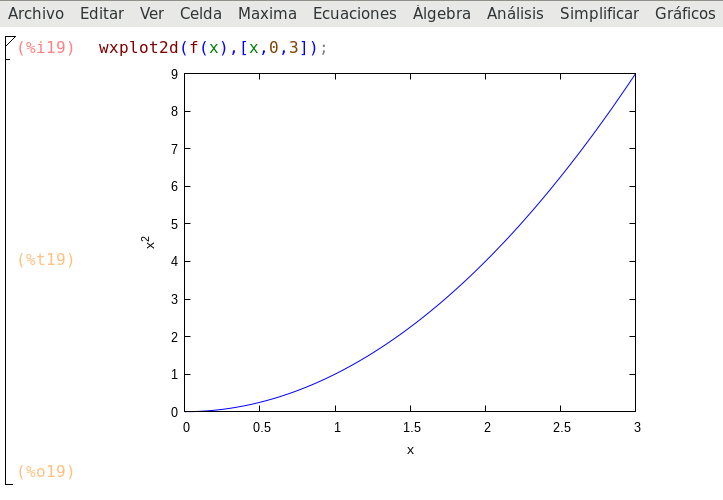
\includegraphics[width=9cm]{graf1.png}
    
\end{center}
\vspace{0.4cm}

Si quieres graficar mas de una función en una gráfica simplemente escribes \textit{wxplot2d([f(x),g(x)],[x,xmin,xmax])}, no necesariamente tienen que ser dos, pueden ser mas, solo sepáralas con una coma.

\begin{center}
	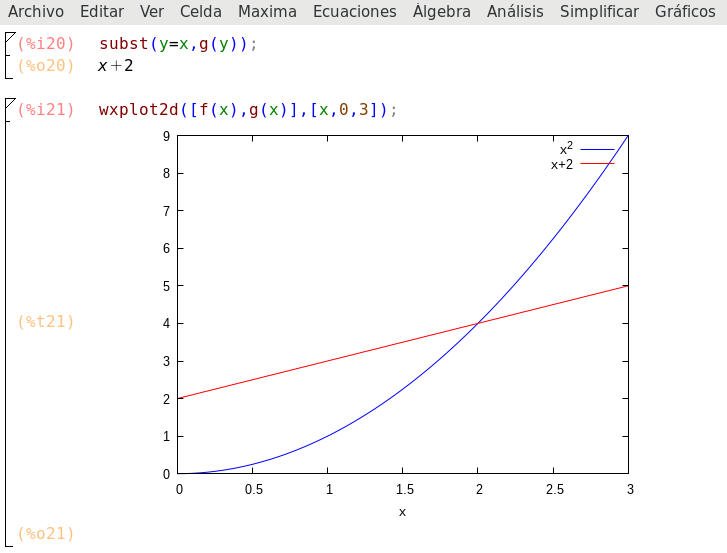
\includegraphics[width=9cm]{graf2.png}
    
\end{center}
\vspace{0.3cm}



\section{Derivar}

Para derivar uno usa el comando \textit{diff()} en donde se escribe la ecuación y la variable a derivar, aquí se muestra un ejemplo: \textit{diff(f(x),x)}

También, uno puede agregar una coma después de la variable a derivar y agregar el orden de derivación para expresar cuantas veces se quiere derivar la función.

\vspace{0.3cm}

Para guardar el resultado en otra función uno puede usar lo siguiente: \textit{g(x):=subst(t=x,diff(f(t),t))}

\vspace{0.3cm}

Ahora, si uno desea el valor numérico solo tiene que sustituir un valor en la función que guardaste al usar el comando de sustitución. 

\begin{center}
	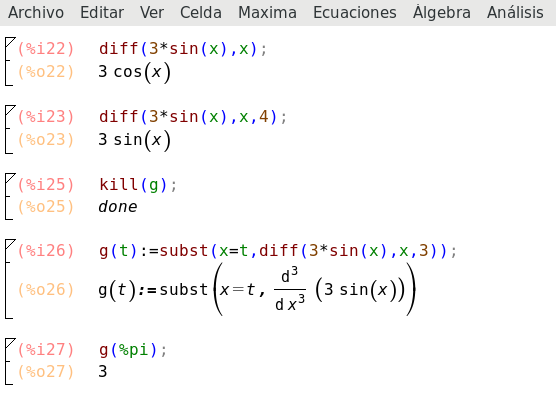
\includegraphics[width=12cm]{deriv.png}
    
\end{center}
\vspace{0.3cm}



\section{Integrar}

Integrar es muy parecido a derivar, simplemente usas el comando \textit{integrate()} e ingresas la función y la variable a integrar, de esta manera: \textit{integrate(f(x),x)}

Para guardar la integral en una función uno tiene que usar el comando de sustitución y sumarle una constante, ya que es una integral indefinida, lo hacemos de la siguiente manera: \textit{f(x):=subst(t=x,integrate(g(t),t))+C}

\vspace{0.3cm}

Cuando uno quiere una integral definida, solo tiene que poner los limites de integración, separados por coma, después de la variable de integración en la misma función de integración, de esta forma: \textit{integrate(f(x),x,a,b)}

\vspace{0.3cm}

En el caso de que uno quiera hacer la integral numérica de una función, simplemente cambia el comando \textit{integrate()} por \textit{quad\_qags()}, pero los que uno ingresa en este es lo mismo que en una integral definida, así: \textit{quad\_qags(f(x),x,a,b)}

EL resultado de esta integral te dará 4 números, el primero es la aproximación de la integral, el segundo es el error máximo que puede tener el resultado, el tercero es información en el numero de funciones cuadráticas que se usaron para aproximar la integral, y el cuarto es un código sobre el tipo de error.

\begin{center}
	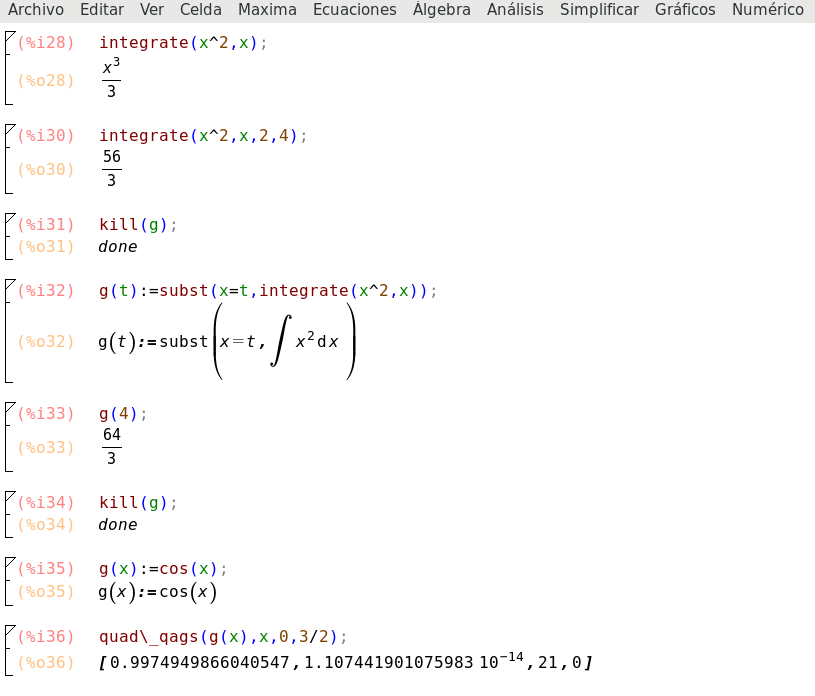
\includegraphics[width=12cm]{int.png}
    
\end{center}
\vspace{0.3cm}



\section{Bilbiografía}

\begin{verbatim}
(n.d.). Retrieved from http://www.scotchildress.com/wxmaxima/ 
\end{verbatim}
%http://www.scotchildress.com/wxmaxima/

\begin{verbatim}
(n.d.). Retrieved from https://def.fe.up.pt/dynamics/maxima_tutorial.
html 
\end{verbatim}
%https://def.fe.up.pt/dynamics/maxima_tutorial.html

\begin{verbatim}
Http://www.avensonline.org/fulltextarticles/JSUR-2332-4139-S1-0001.
html. (2015). Journal of Surgery, 01-07. doi:10.13188/2332-4139.s100001 
\end{verbatim}
%http://maxima.sourceforge.net/docs/manual/maxima_singlepage.html#SEC_Top



\section{Apéndice}


    1.- ¿Cuál fue tu primera impresión de wxmaxima?
    
    \vspace{0.3cm}
		Me pareció a Python solo que sin muchas maneras de personalizar lo que quieres hacer, pero menos complicado para obtener ciertas cosas.
    \vspace{0.3cm}
    
\noindent 2.- ¿Crees que esta herramienta puede ser útil en otros de tus cursos?
    
    \vspace{0.3cm}
 		Si
    \vspace{0.3cm}
    
\noindent    3.- ¿Qué se te dificultó mas en esta actividad?
    
    \vspace{0.3cm}
		En general no fue difícil, solo fue un poco larga.
    \vspace{0.3cm}
    
\noindent    4.- ¿Se te hizo compleja esta actividad? ¿Cómo la mejorarías? 
    
    \vspace{0.3cm}
		Esta actividad no me pareció muy complicada, me pareció perfecta para la semana de evaluación. 
    \vspace{0.3cm}


\end{document}